\section{\acl{LSTM}}
\textit{Daniel Andrés López, Frank Reichwein}

\ac{LSTM} ist ein \ac{RNN}, welches die Eigenschaft hat Zustände über einen
bestimmten Zeitraum zu behalten und danach wieder zu vergessen. \acp{LSTM} sind
somit eine spezielle Form von \acp{MLP}. Ein \ac{LSTM} definiert rekurrente
Verbindungen (Verbindungen von Neuronen zu vorhergehenden bzw. denselben
Neuronen) in der Art und Weise, dass die Eingabe Daten bzw.
die Ausgabe Daten gespeichert über mehrere Aufrufe des Netzwerkes hinaus
gespeichert werden. Diese gespeicherten Daten werden bei bestimmten
Eingangsdaten ausgegeben, bei anderen \textit{vergessen} bzw. überschrieben oder
nicht verwendet. 
  
\acp{RNN} und vielmehr noch \acp{LSTM} sind Modelle für das menschliche Gehirn.
Im Gehirn sind viele Neuronen untereinander, also mit sich selbst, nachfolgenden
und vorhergehenden Neuronen vernetzt, sogenannten Feedback Verbindungen. Jedes
Neueron ist dabei ein speziell aufgebaut um Informationen zu speichern.
\acp{RNN} haben keine bzw. einfache Erinnerungsneuronen und sind aus diesem
Grund nicht für länger Erinnerungen geeignet. Bei \acp{LSTM} hingegen sind
komplexe Erinnerungsneuronen (\ac{LSTM}-Neuronen) miteinander verknüpft. Jedes
einzelne Neuron kann Informationen über einen längeren Zeitraum, d.h. auch bei
häufiger Nutzung des Netzes, Daten speichern. Dadurch dass \acp{LSTM} Daten auch
nach dem Training speichern können, also verschiedene Zustände haben,
unterscheiden sie sich von vielen anderen Machine Learning Verfahren, wie z.B.
\ac{HMM} oder \acp{SVM}. Sie sind besonders für komplexe Aufgaben mit unscharfen
Beobachtungen geeignet und werden bevorzugt in Handschrift- und Spracherkennung,
Proteinanalyse und weiteren dynamischen Feldern verwendet. Durch die Analogie
zum Gehirn können \acp{LSTM} biologisch motiviert werden.
 
\subsection{Architektur von \aclp{LSTM}}
Ein \ac{RNN} mit \ac{LSTM} Einheiten hat ein Hiddenlayer in dem die
verschiedenen \ac{LSTM} Knoten enthalten sind. Das Outputlayer ist dann ein
einfaches lineares oder sigmoidales Layer. 
 
\begin{figure}[htfp]
	\begin{center}
	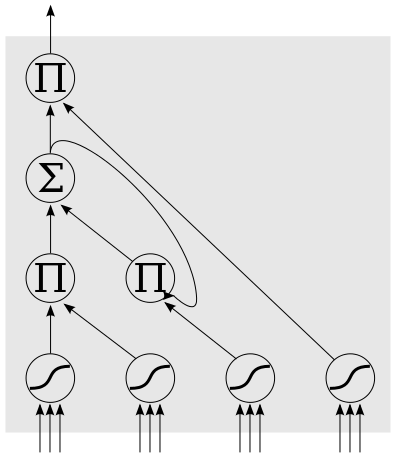
\includegraphics[width=0.3\textwidth]{lstm_block}
	\caption{Schema eines \acs{LSTM} Blocks}
	Quelle: \cite{WIKI2013}
	\label{fig:lstm_block}
	\end{center}
\end{figure}

In \autoref{fig:lstm_block} ist das Schema eines \ac{LSTM} dargestellt. sind die
verschiedenen Knoten in der unteren Zeile folgendes: Input, Input Gate, Forgot
Gate, Output Gate. Die drei Gates bestimmen ihrem Namen entsprechend, ob der
Input in den Block hineingelassen wird, ob der vorhandene Datensatz vergessen
werden soll oder ob das Datum ausgegeben werden soll. Der erste Knoten dient zur
Verarbeitung der Inputwerte. Die $\Pi$ Knoten sind zur Berechnung der
entsprechenden Werte:

links in der zweiten Zeile ist zur Weitergabe des verarbeiteten Inputwertes
(bei Aktivierung durch das Input Gate wird dieser weitergereicht); der rechte
$\Pi$ Knoten reicht entweder den gespeicherten Wert des $\Sigma$ Knotens weiter
oder einen Initialwert bei Aktivierung des Forgot Gates; Der $\Pi$ Knoten in der
obersten Zeile dient der Weitergabe des gespeicherten Wertes, falls das Output
Gate aktiviert ist, andernfalls erfolgt keine Aktivierung dieses Knotens. Im
$\Sigma$ Knoten wird der Wert gespeichert und durch eine Rückverbindung über
mehrere Schritte erhalten. Wird das Input Gate aktiv, wird $\Sigma$ durch den
verarbeiteten Input ersetzt, mit einem aktiven Forgot Gate \textit{gelöscht}. 


\subsection{Funktionsweise von der \acs{PyBrain} \acs{LSTM} Implementierung}
\ac{PyBrain}\cite{schaul2010} ist eine Bibliothek für Python und stellt
verschiedene Module aus dem Bereich des maschinellen Lernes bereit. Dabei
spielen neuronale Netzwerke eine zentrale Rolle, diese werden in verschiedenen
Lernmethoden angewendet wie z.B. im Reinforcement, unüberwachten oder
evolutionären Lernen.

\begin{lstlisting}[caption={Aufbau eines LSTM Netzes},label={lst:lstm_example}]{lst:lstm_example} 
net = buildNetwork(INPUTS, HIDDEN, OUTPUTS, hiddenclass=LSTMLayer,
outclass=SigmoidLayer, recurrent=True, bias=True) 
ds = DATASET 
trainer = BackpropTrainer(net, ds)
for _ in range(1000):
    trainer.train()
\end{lstlisting}

In \autoref{lst:lstm_example} ist ein Beispiel aufgezeigt wie \ac{PyBrain}
verwendet werden kann. Es gibt dabei verschiedene Möglichkeiten im Aufbau des
Netzes (v.a. Anzahl der Neuronen und \ac{LSTM}-Blocks), in der Datenhaltung
(\ref{sec:lstm_data}) sowie in der Trainingsmethode (z.B. Backpropagation).
Die \ac{PyBrain} Implmenetierung bringt bereits die Umsetzung der
\ac{LSTM}-Blocks mit, sodass die konkrete Umsetzung der Blöcke nicht
durchgeführt werden muss.

\subsection{Verwendetes Datenmodell}
\label{sec:lstm_data}

Im \autoref{sec:gestures_dataformat} wird beschrieben wie Gesten aufgenommen und
abgespeichert werden. Dabei wird ein Trainingsdatenset erzeugt, dass für
jeden Datensatz eine bestimmte Anzahl an Frames mit je 64 Datenpunkte im
gewünschten Frequenzbereich enthält. 

Für das \ac{LSTM} Netz wird jeder Datensatz als linear aus den einzelnen Frames
aufgebaut. Dadurch entsteht ein einzelner Eingabevektor inkl. der
Klassifizierung. Zur Vereinheitlichung und Vergleichbarkeit werden die Daten
noch normalisiert.
Dies ist notwendig, da Datensätze unter verschiedenen Bedingungen erzeugt werden
können, z.B. im lauten Umfeld, andere Anordnung von Mikrofon und Lautsprecher,
unterschiedlicher Größe der Hände, unterschiedliche Lautstärke, etc. Um
vergleichbare Daten zu erhalten wird daher die Amplitude der Referenzfrequenz
als Normailisrungsfaktor verwendet, diese ist i.d.R. am größten. Durch diese
Normalisierung der Referenzfrequenz auf 1 werden alle weiteren Datenpunkte im
Intervall zwischen 0 und 1 liegen. Eine weitere Möglichkeit die es zu
untersuchen gilt, ist die Betrachtung der Abweichung der Amplituden im Verlauf
der Geste im Vergleich zu einem Frame ohne Geste. Diese Änderungen pro Frame
können dann anstatt der Originaldaten gelernt werden. Alternativ kann zur
Unterscheidung von Gesten vom Hintegrundrauschen noch ein Datenset mit
Hintergrundrauschen genutzt werden. Hier muss sich noch zeigen wie gut das
\ac{LSTM} Netz ohne diese Daten klassifiziert, je nach Ergebnis wird es noch
hinzugezogen. 

Durch die Erinnerungsmöglichkeit des \ac{LSTM} Netzes ist es möglich die die
Frames in einer einzeln (d.h. lediglich die 64 Datenpunkte an einem Zeitpunkt)
in das Netzwerk gegeben werden. Die \ac{LSTM}-Blöcke merken sich dann jeweils
die verschiedenen vorherigen Eingabedaten und werden daran dann die
entsprechende Klasse bei neuen Eingaben erkennen. Dazu ist es dann auch nicht
mehr notwendig, dass die Gestenaufnahme diskret abläuft (je 0,5 Sekunden dem
Klassifikator zur Verfügung stellen), sie kann auch kontinuierlich ablaufen,
d.h. jedes neu aufgenommene Frame kann sofort weitergegeben werden und wird vom
Netz verarbeitet. Mit dem richitgen Erinnerungszeitraum, erkennt das Netz dann
die Gesten direkt hintereinander bzw. ineinander übergehend. Diese Idee gilt es
noch zu überprüfen, insbesondere auf die technische Umsetzung (PyBrain
Parameter korrekt setzen).




\nocite{GERS2001,WIKI2013,Schmidhuber2013,LSTM1,Nerbonne1}
